\chapter{Methodology for Image Registration}
\label{section:methodology-for-image-registration}

This chapter describes the methodology for image registration, that is, the process that colorizes (defines the colors) the point cloud based on the images taken in the acquisitions. This method can be split into two parts: the Color Registration (\cref{section:color-registration}), where the process is described per-image and each image colorizes a portion of the point cloud, and the Color Fusion (\cref{section:color-fusion}), where all the colorized point cloud are merged into the final colorized point cloud. The pixel registration relies on a camera calibration, both the intrinsic calibration and also the extrinsic, so two methods are shown to obtain this calibration (\cref{section:camera-intrinsic-calibration,section:camera-extrinsic-calibration}).

\section{Color Registration}
\label{section:color-registration}

This method describes how to colorize a point cloud based on a single image, using projection principle based on the camera model. As an overview, each point in the point cloud can be projected as a ray in the camera perspective, which is basically the path from the eye point to the point. This ray can be used to retrieve the original color of the point from the image. However, this process is not so straightforward, because the position and orientation of the camera has to be very precise and occlusion has to be considered.

\subsection{Point Projection}

To start with, each point has to be transformed, because the original point is registered in the scene coordinate frame ($p_{scene}$) and has to be transformed into the camera coordinate frame ($p_{camera}$). So, the transformations $\prescript{acquisition}{scene}{T}$, $\prescript{ptu}{acquisition}{T}$, $\prescript{camera}{ptu}{T}$ can be used according to \cref{eqn:point-camera-transformation}. The $\prescript{acquisition}{scene}{T}$ transformation is obtained in \cref{section:acquisition-registration}, $\prescript{ptu}{acquisition}{T}$ is the transformation of the PTU and $\prescript{camera}{ptu}{T}$ is the extrinsic calibration of the camera and the method to obtain it is in \cref{section:camera-extrinsic-calibration}. The transformation graph can be seen in \cref{fig:color-registration-3d}.

\begin{equation}
    \label{eqn:point-camera-transformation}
    p_{scene} =
        \prescript{acquisition}{scene}{T} \cdot 
        \prescript{ptu}{acquisition}{T} \cdot
        \prescript{camera}{ptu}{T} \cdot p_{camera}
\end{equation}

\begin{figure}
    \tdplotsetmaincoords{70}{150}
    \centering
    \begin{tikzpicture}[tdplot_main_coords]

        \coordinate (scene) at (-4,0,0);
        \coordinate (acquisition) at (7, 5, 5);
        \coordinate (ptu) at (10, 5, 7);
        \coordinate (camera) at (8, 7, 10);

        \tikzset{
            axes/.pic = {
                \draw[thick,->] (0,0,0) -- +(-1,0,0) node[anchor=west]{$y$};
                \draw[thick,->] (0,0,0) -- +(0,1,0) node[anchor=west]{$x$};
                \draw[thick,->] (0,0,0) -- +(0,0,1) node[anchor=south]{$z$};
            }
        };

        \newcommand{\axes}[1] {
            \draw[thick,->] #1 -- +(-1,0,0) node[anchor=west]{$y$};
            \draw[thick,->] #1 -- +(0,1,0) node[anchor=north west]{$x$};
            \draw[thick,->] #1 -- +(0,0,1) node[anchor=south]{$z$};
        }

        \draw pic at (scene) {axes};
        \node[below left, scale=0.7] at (scene) {scene};

        \draw pic at (acquisition) {axes};
        \node[below left, scale=0.7] at (acquisition) {acquisition};

        \tdplotsetrotatedcoords{0}{0}{30}
        \draw[tdplot_rotated_coords] pic at (ptu) {axes};
        \node[below left, scale=0.7] at (ptu) {ptu};

        \tdplotsetrotatedcoords{10}{-85}{0}
        \draw[tdplot_rotated_coords] pic at (camera) {axes};
        \node[above left, scale=0.7] at (camera) {camera};

        \path[-latex]
            (scene) edge[bend right=10] node[midway, above] {$\prescript{acquisition}{scene}{\mathcal{T}}$} (acquisition)
            (acquisition) edge[bend left=20] node[midway, below left] {$\prescript{ptu}{acquisition}{\mathcal{T}}$} (ptu)
            (ptu) edge[bend left=20] node[midway, above left] {$\prescript{camera}{ptu}{\mathcal{T}}$} (camera);

        \draw[tdplot_rotated_coords]
            ($(camera) + ( 0.8, 1, 3)$) -- 
            ($(camera) + ( 0.8,-1, 3)$) -- 
            ($(camera) + (-0.8,-1, 3)$) --
            ($(camera) + (-0.8, 1, 3)$) -- cycle;
        \draw[tdplot_rotated_coords, -latex, thick]
            ($(camera) + ( 0.8, -1, 3)$) -- +(0, 2.5, 0)
            node[above] {$u$};
            \draw[tdplot_rotated_coords, -latex, thick]
            ($(camera) + ( 0.8, -1, 3)$) -- +(-2, 0, 0)
            node[below] {$v$};
        
        \coordinate (point) at (0, 6, 10);
        
        \coordinate (projected) at ($0.35*(point)+{1-0.35}*(camera)$);
        \node[tdplot_rotated_coords, scale=2]
            at (projected)
            {$.$};
        \node[tdplot_rotated_coords, scale=0.6, above]
            at (projected)
            {$(u_i,v_i)$};

        \node[scale=2] at (point) {$.$};
        \node[above right] at (point) {$p_i$};

        \draw[-latex] (camera) -- (point);

        
    \end{tikzpicture}

    \caption{Color registration for a single point.}
    \label{fig:color-registration-3d}
\end{figure}

Next, each point was transformed into pixel coordinates $(u, v)$, using the pinhole camera model. This model defined how a light ray in projected in the image sensor of a camera and has two parameters: the focal length $f = (f_x, f_y)$ and optical center $(c = (c_x, c_y))$. This parameters are obtained in the intrinsic calibration of the camera (\cref{section:camera-intrinsic-calibration}). According to this model, each point is projected as pixel coordinates $(u, v)$ to a plane located a unit distance from the camera eye point, using the perspective projection matrix in \cref{eqn:perspective-matrix}, according to:

\begin{equation}
    \label{eqn:perspective-matrix}
    \mathcal{P} =
    \left[
        \begin{array}{ccc}
            f_x & 0   & c_x \\
            0   & f_y & c_y \\
            0   & 0   & 1   \\
        \end{array}    
    \right],
\end{equation}

\begin{equation}
    \label{eqn:perpective-transformation}
    \left(
        \begin{array}{c}
            u z \\ v z \\ z \\
        \end{array}    
    \right)
    =
    \mathcal{P} \cdot
    \left(
        \begin{array}{c}
            x \\ y \\ z \\
        \end{array}    
    \right).
\end{equation}

The pinhole camera model does not regard the distortion caused by the lens, which is not negligible for most cameras. The two sources of distortion are radial and tangential distortion. Radial distortion makes straight lines appear curved, known as the barrel distortion and pincushion distortion. This distortion is highly noticed in images taken with fish-eye lenses, as seen in \cref{fig:fisheye}. This distortion can be solved by transforming the $(u, v)$ with \cref{eqn:radial-distortion}. Similarly, tangential distortion is caused by a misalignment of the lens to the imaging plane, which causes areas in the image to appear closer than expected. This deformation can be solved with the \cref{eqn:tangential-distortion}. In brief, to undistort the image five parameters need to be determined, also known as the distortion coefficients: $\{k_1, k_2, p_1, p_2, k_3\}$, which are obtained in the camera intrinsic calibration method, described in \cref{section:camera-intrinsic-calibration}.

\begin{align}
    \label{eqn:radial-distortion}
    \left(
        \begin{array}{c}
            u \\ v \\
        \end{array}
    \right)_{calibrated}
    & =
    (1 + k_1 r^2 + k_2 r^4 + k_3 r^6)
    \left(
        \begin{array}{c}
            u \\ v \\
        \end{array}
    \right).
    \\
    \label{eqn:tangential-distortion}
    \left(
        \begin{array}{c}
            u \\ v \\
        \end{array}
    \right)_{calibrated}
    & =
    \left(
        \begin{array}{c}
            u \\ v \\
        \end{array}
    \right)
    + 
    \left(
        \begin{array}{c}
            2 p_1 u v + p_2 (r^2 + 2u^2) \\
            p_2 (r^2 + 2v^2) + 2 p_2 u v \\
        \end{array}
    \right).
\end{align}

\begin{figure}[h]
    
    \centering
    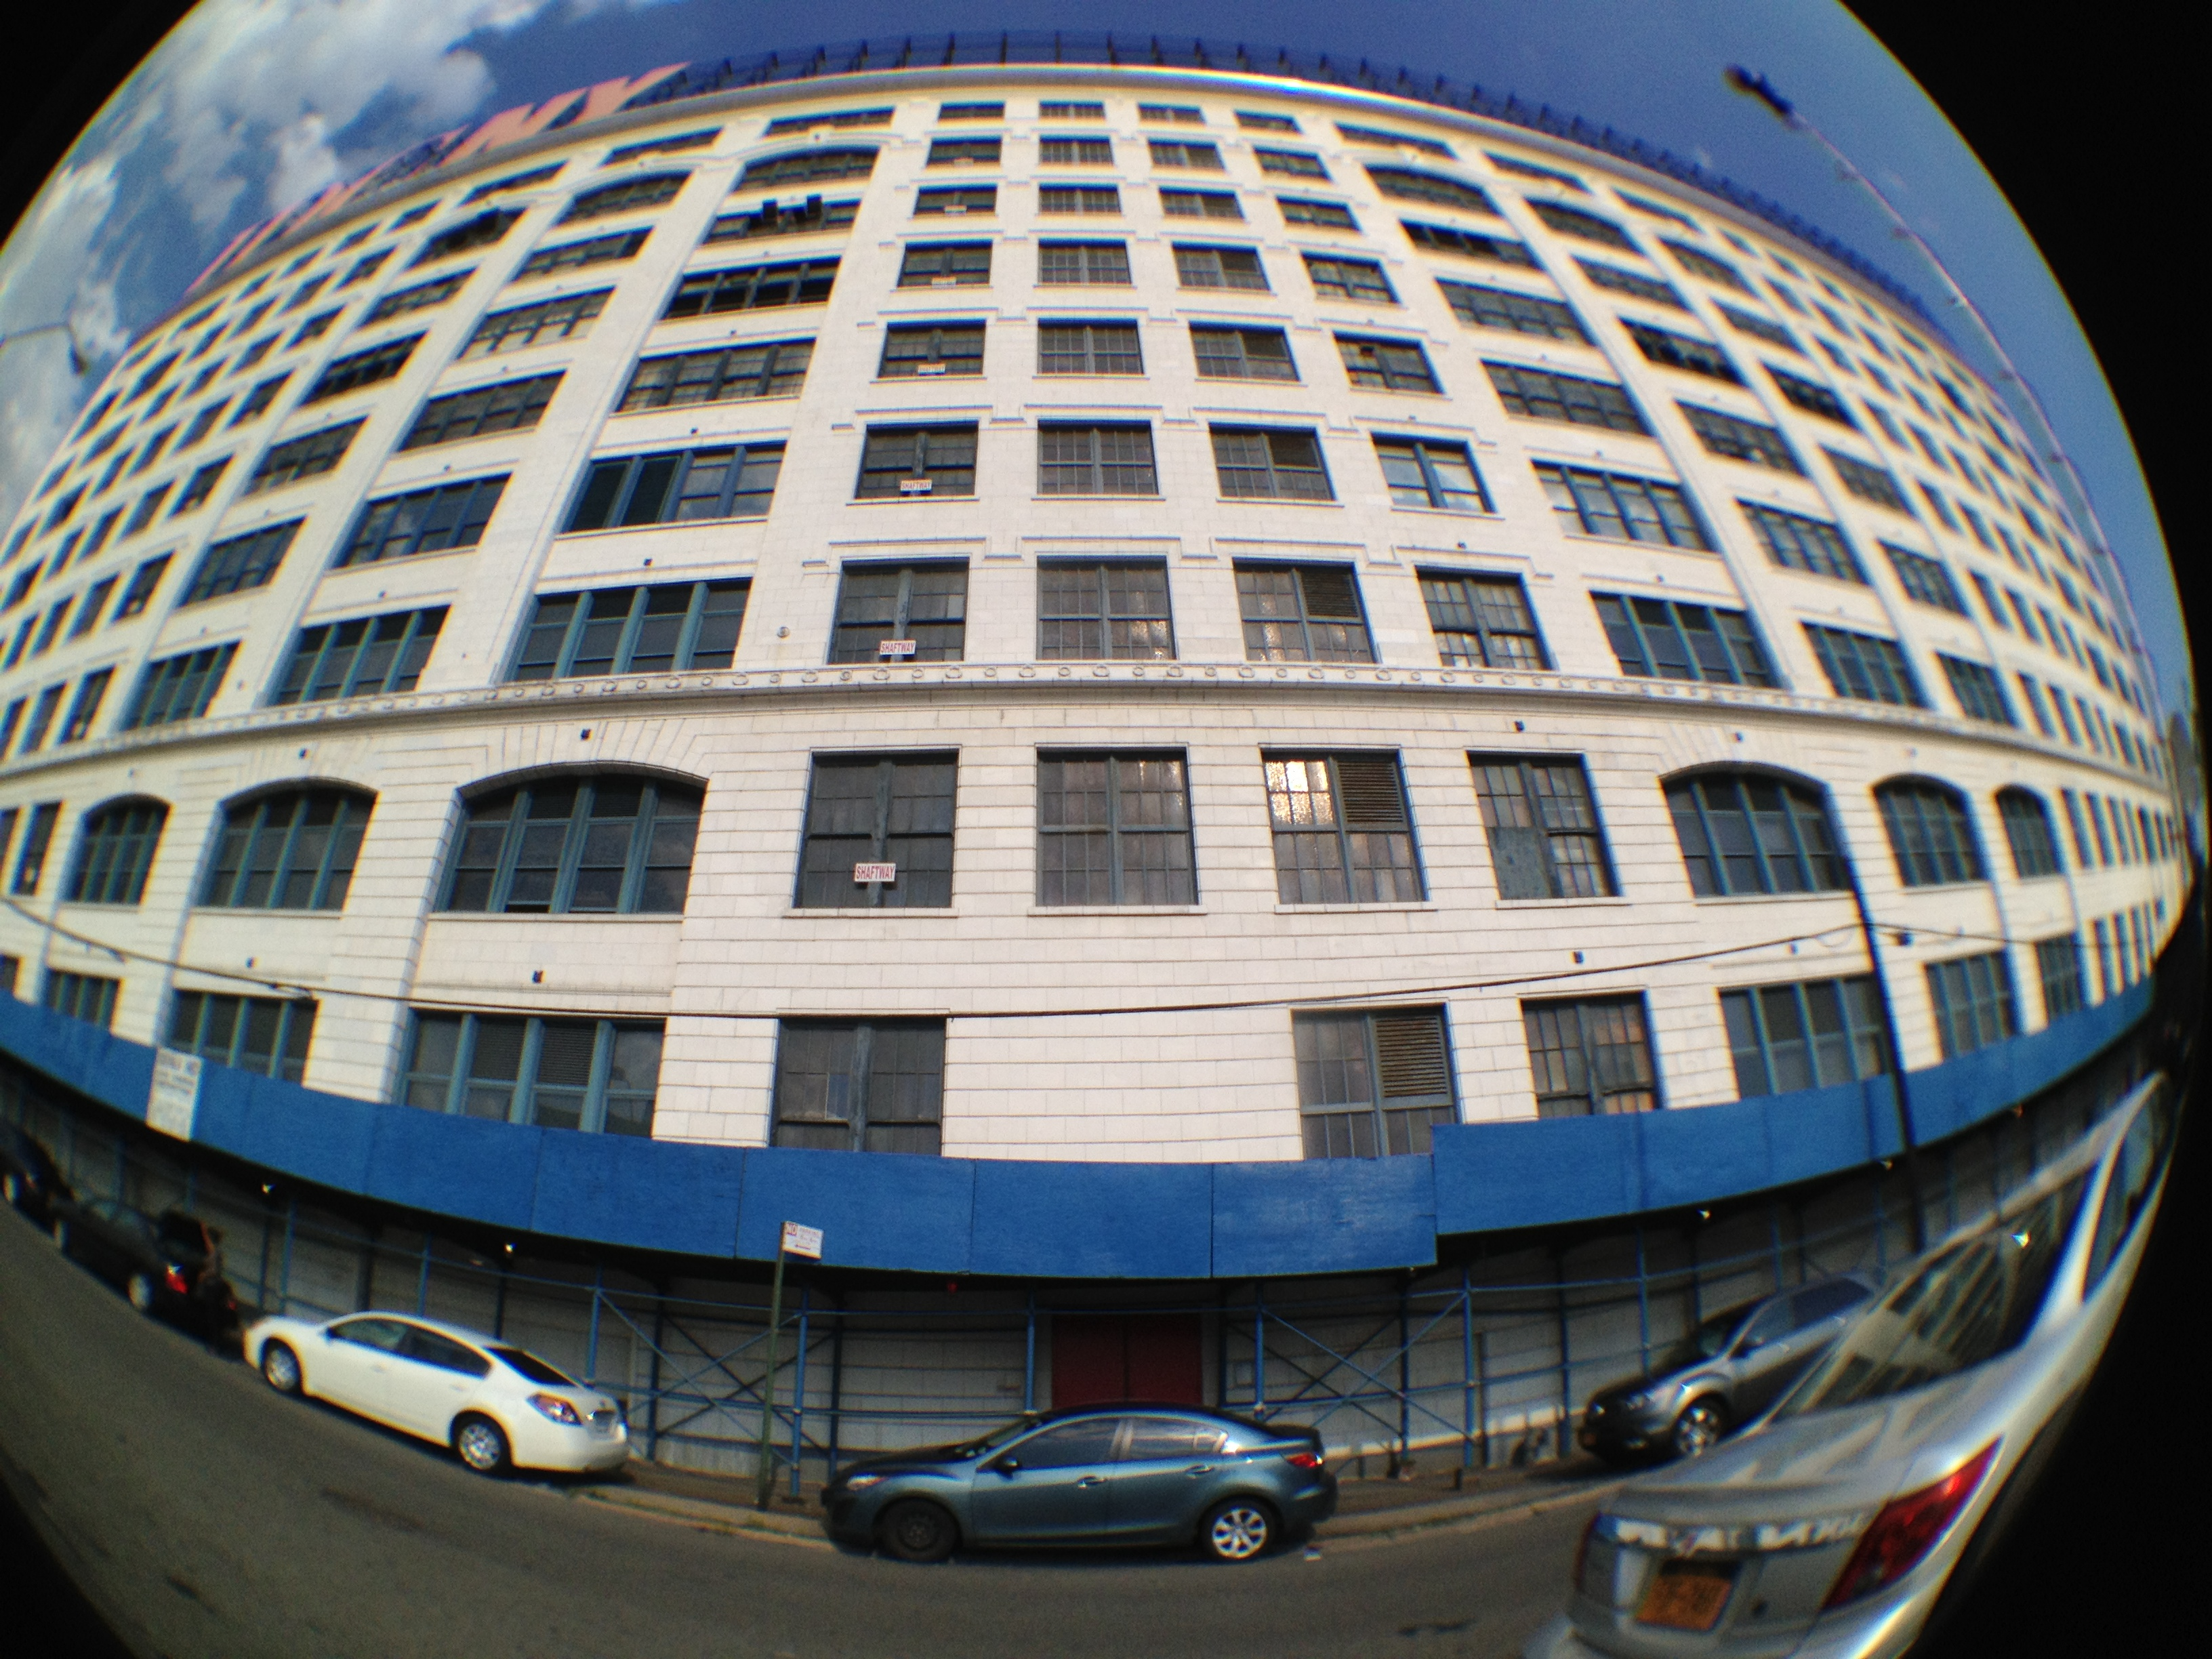
\includegraphics[width=0.65\textwidth]{fisheye}

    \caption{Barrel distortion in fish eye lens.}
    \label{fig:fisheye}

\end{figure}

\subsection{Camera Intrinsic Calibration}
\label{section:camera-intrinsic-calibration}

The intrinsic calibration determines the intrinsic parameters of the camera. The calibration procedure used in this work is a standard procedure for cameras with low distortion and is known as the chessboard camera calibration. This method calibrates a monocular camera with fixed focus using a sequence of images taken from a chessboard with known dimensions.

In order to improve the calibration results, the chessboard should rotate and move, in order to occupy the entire image size and the chessboard poses should be enough and be well distributed spatially. Also, the calibration is more accurate if the corners of the chessboard are well defined in the image, so the chessboard should have an appropriate size

In the end, the accuracy of the calibration should be measured for new images, with the re-projection error. This value should be as low as possible and, as a rule of thumb, a value less than \num{0.01} is acceptable.

In ROS, this calibration is easily obtained with the \emph{cameracalibrator.py}, which includes a graphical interface, and provides feedback about the corner detection and the state of the calibration. The interface is shown on \cref{figure:camera-calibrator}. In this system, this data is first saved into a ROS \emph{camera\_info} file. Then, this file is also saved in each capture in the parameters file.

\begin{figure}
    
    \centering
    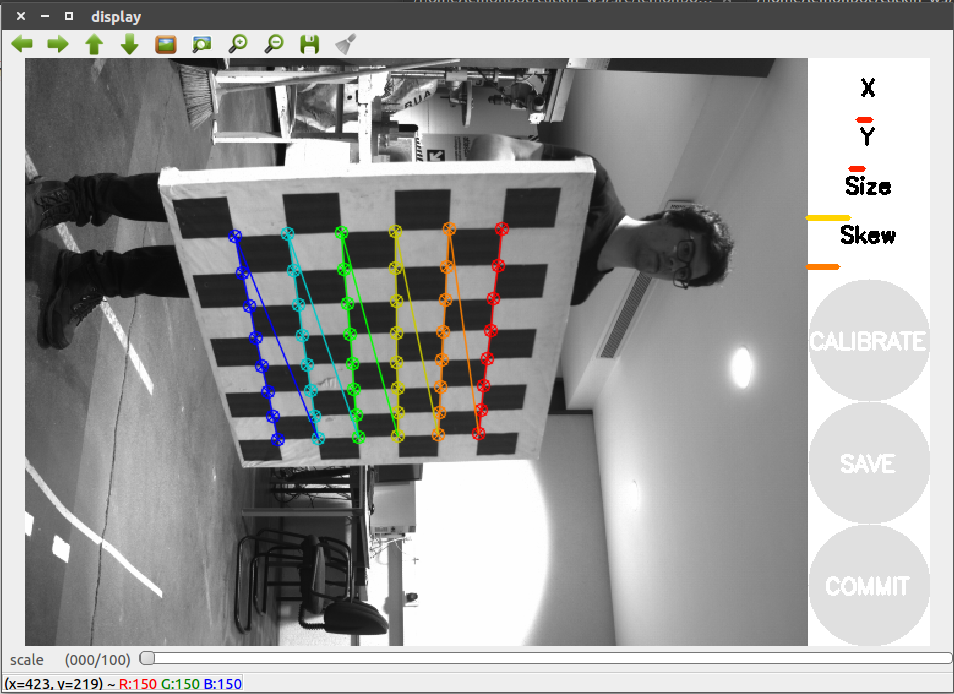
\includegraphics[width=10cm]{camera-intrinsic-calibration}

    \caption{Interface for the \emph{cameracalibrator} node.}
    \label{figure:camera-calibrator}

\end{figure}

\subsection{Camera Extrinsic Calibration}
\label{section:camera-extrinsic-calibration}

The calibration method used to determine the extrinsic parameters is known as the eye-in-hand calibration, described in \cite{horaud95}.

This calibration relies on a static calibration object, whose pose can be estimated in the camera frame. Hence, four coordinate frames and four transformation exist. The four frames are the \emph{camera} frame, the \emph{world} frame, the \emph{PTU} frame and the \emph{object}. The four transformations are the extrinsic transformation of the camera, or the \emph{PTU} to the \emph{camera} transformation $\TF{ptu}{camera}$, which is static and unknown, the \emph{camera} to \emph{object} transformation $\TF{camera}{object}$, which is obtained by the object pose estimation algorithm, the \emph{world} to \emph{PTU}, which is known and, finally, the \emph{world} to \emph{object} transformation, which is static and unknown. The overall transformation graph is shown is in \cref{fig:hand-in-eye-tf-graph}, with the unknown transformations in red and the known transformations in green.

\begin{figure}
    
    \centering
    \begin{tikzpicture}
        \node[draw, ellipse] (world) at (0,0) {world};
        \node[draw, ellipse] (hand) at (-4,3) {hand/ptu};
        \node[draw, ellipse] (object) at (4,3) {object};
        \node[draw, ellipse] (camera) at (0, 6) {camera};
        
        \path[-latex]
            (world) edge[bend right] node[midway, below right, red] {$\TF{world}{object}$} (object)
            (world) edge[bend left] node[midway, below left, blue] {$\TF{world}{ptu}$} (hand)
            (hand) edge[bend left] node[midway, above left, red] {$\TF{hand}{camera}$} (camera)
            (camera) edge[bend left] node[midway, above right, blue] {$\TF{camera}{object}$} (object);
    \end{tikzpicture}

    \caption{Hand-in-eye transformation graph.}
    \label{fig:hand-in-eye-tf-graph}

\end{figure}

The inspection of the transformation graph determines an equality, because there are two possible ways to transverse the graph from one node to another, which yields the \cref{eqn:hand-in-eye-equality}. This equality is the base of this optimization: $\TF{ptu}{camera}$ can be obtained from multiple pairs of synchronized $\TF{world}{object}$ and $\TF{camera}{object}$ transformations.

\begin{equation}
    \label{eqn:hand-in-eye-equality}
    \TF{world}{object} = \TF{world}{ptu} \cdot \TF{ptu}{camera} \cdot \TF{camera}{object}
\end{equation}

In this work, the object used for detection was an ArUco marker, which is comprised of a pattern which can be detected and also allows for precise pose estimation, as seen in \cref{fig:aruco-detection}. One of the biggest advantages over other markers is that the implementation for detection and pose estimation is already implemented in the ROS package \emph{aruco\_detect}. The calibration is also implemented in the ROS package \emph{visp\_hand2eye\_calibration}, as a node that receives multiple transformations in the topics \emph{/world\_effector} and \emph{/camera\_object}, which correspond respectively to the $\TF{world}{ptu}$ and $\TF{camera}{object}$ transformations. To publish the transformations on this topics, a node was developed, the \emph{hand2eye\_simple\_client}, which publishes both the transformations synchronously at the keypress of the user. The control of the PTU was also manual. 

\begin{figure}
    
    \centering
    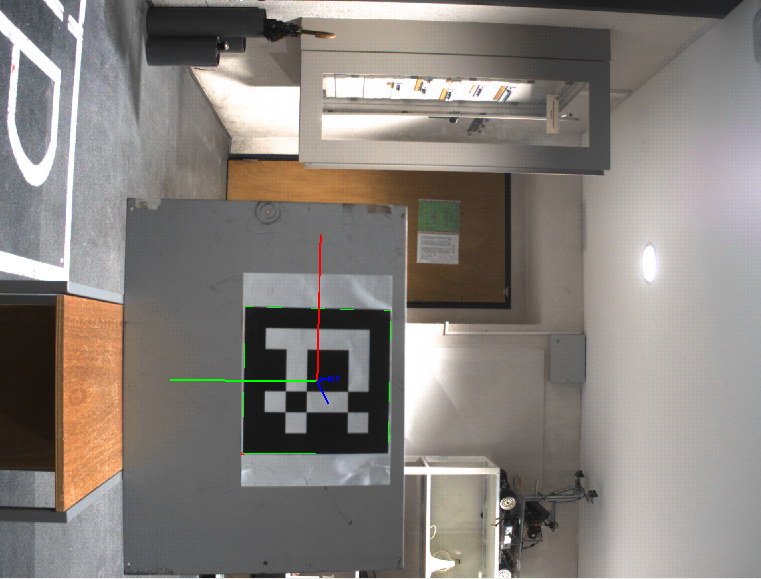
\includegraphics[width=10cm]{camera-extrinsic-calibration}

    \caption{ArUco maker detection and pose estimation.}
    \label{fig:aruco-detection}
\end{figure}

\subsection{Point filtering}

Not all points are eligible for the color registration, based on it's location and camera properties, so two filtering steps were used: the first filter removes the points outside the field of view and the second removes the occluded points.

\subsubsection{Field of View Removal Filter}

The field of view is defined as the region of space that is captured by the camera sensor, which for pinhole cameras has a pyramid geometry, as seen in \cref{fig:camera-fov}. The sides of the pyramid are limited by the size of the sensor, so the points that lie outside the rectangle defined by the points $(0,0)$ and $(width, height)$ are excluded, as:


\begin{equation}
    \label{eqn:frustum-condition}
    \begin{aligned}
                 & 0        & < u & < width \\
        \wedge \ & 0        & < v & < height. \\
    \end{aligned}
\end{equation}


\begin{figure}[h]
    
    \tdplotsetmaincoords{70}{140}
    \centering
    \begin{tikzpicture}[tdplot_main_coords]
        \coordinate (eye) at (0,0,0);

        \node[above left, scale=0.7] at (eye) {eye point};

        \draw[thick,->] (eye) -- +(-10,0,0) node[anchor=north west]{$z$};
        \draw[thick,->] (eye) -- +(0,1,0) node[anchor=north west]{$x$};
        \draw[thick,->] (eye) -- +(0,0,-1) node[anchor=north]{$y$};

        \newcommand{\drawfrustumlines}[2]{
            \def\x{#1/#2};
            \draw[dashed] (eye) -- (#1, \x, \x);
            \draw[dashed] (eye) -- (#1, -\x, \x);
            \draw[dashed] (eye) -- (#1, \x, -\x);
            \draw[dashed] (eye) -- (#1, -\x, -\x);
        }
        \newcommand{\drawfrustum}[3]{
            \def\a{#1/#3};
            \def\b{#2/#3};
            \draw (#1, \a, \a) -- (#1, -\a, \a) -- (#1, -\a, -\a) -- (#1, \a, -\a) --cycle;
            \draw (#2, \b, \b) -- (#2, -\b, \b) -- (#2, -\b, -\b) -- (#2, \b, -\b) --cycle;
            \draw (#1, \a, \a) -- (#2, \b, \b);
            \draw (#1, -\a, \a) -- (#2, -\b, \b);
            \draw (#1, -\a, -\a) -- (#2, -\b, -\b);
            \draw (#1, \a, -\a) -- (#2, \b, -\b);

        }

        \drawfrustumlines{-10}{8};
        \drawfrustum{-8}{-4}{8};

        % \draw[dashed] (0,0,-1.5) -- (0,0, -2);
        % \draw[dashed] (-4,0,-2) -- (-4, 0, -1);
        % \draw[dashed] (-8,0,-2) -- (-8, 0, -1.5);

        % \draw[latex-latex] (0,0,-2) -- (-4, 0, -2) node[above, midway, sloped] {$z_{near}$};
        % \draw[-latex] (-4,0,-2) -- (-8, 0, -2) node[above, midway, sloped] {$z_{far}$};
        
    \end{tikzpicture}

    \caption{Representation of the visual frustum of the camera.}
    \label{fig:camera-fov}

\end{figure}

\subsubsection{Hidden Point Removal Filter}

Not all points that lie on the frustum of the camera are seen by the camera, because some of this points are occluded by nearer objects, so they need to be removed. A fast and straightforward solution is to use the point cloud resulting from the same acquisition as the image, because the sensor are considered close together. However, this is not the best solution, as it would be better if the point cloud obtained after the acquisition registration was used.

In \cite{katz07}, an simple and fast operator, the Hidden Point Removal, or HPR, determines the visibility of point sets, viewed from a given viewport. This method is easily implemented and has a asymptotic complexity of $O(n \log n)$, where $n$ is the number of points in the point cloud. Moreover, this method works well for both sparse and dense point clouds.

The HPR operator operates on a set of points $\mathcal{P} = \{p_i | i = 1 \dots n \}$, and the goal is to determine whether $p_i$ is visible from a viewpoint $\mathcal{C}$. In this application, $C$ is the origin of the point cloud. The algorithm consists of two steps: the inversion and the construction of the convex hull.

The inversion step maps each point $p_i$ along the ray from $\mathcal{C}$ to $p_i$, such that $|p_i|$ is monotonically decreasing. There are multiple ways to perform the inversion, but in \cite{katz07} the \emph{spherical flipping} was used. Spherical flipping reflects a point $p_i$ with respect to a sphere of radius $R$ to the new point $\hat{p_i}$ by applying:

\begin{equation}
    \label{eqn:spherical-flipping}
    \hat{p_i} = p_i + 2 (R - |p_i|) \frac{p_i}{|p_i|}.
\end{equation}

Afterwards, the convex hull of $\hat{\mathcal{P}} \bigcup \{\mathcal{C}\}$, where $\hat{\mathcal{P}}$ is the transformed point set and $\mathcal{C}$ is the center of the sphere, is computed. Finally, the points that lie in the convex hull are the visible points of the point set.

This algorithm only has a parameter, which is the radius $R$ of the sphere used for the spherical flipping, which influences the amount of false positives of the algorithm. In general, $R$ is determined based on the maximum point length $max(|p_i|)$ and a exponential factor $\alpha$, such that $R = max(|p_i|) \times 10^{\alpha}$. In this application, a factor of $\alpha = 3$ was empirically selected.

As an example, the HPR operator was used in the Stanford Bunny\footnote{From https://www.cc.gatech.edu/~turk/bunny/bunny.html.} point cloud, as seen in \cref{fig:hpr-operator-bunny} and, as seen, \cref{fig:after-hpr} only presents the points that are visible, as opposed to \cref{fig:before-hpr}.

\begin{figure}[h]
    
    \centering
    \begin{subfigure}{0.5\textwidth}
        \centering
        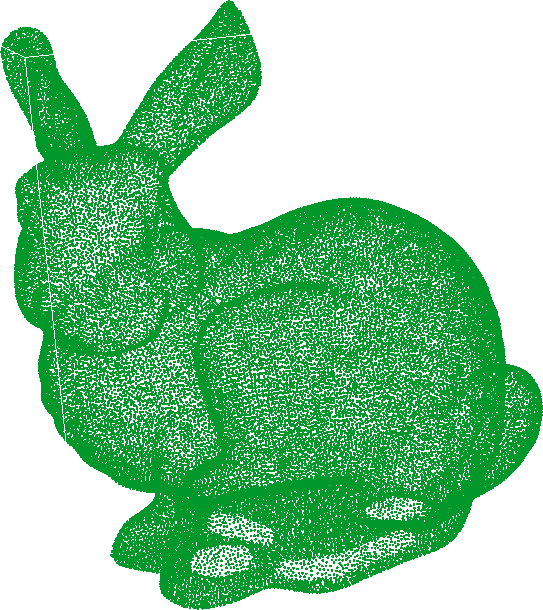
\includegraphics[height=6cm]{bunny-before-hpr}
        \caption{Before the HPR.}
        \label{fig:before-hpr}
    \end{subfigure}%
    \begin{subfigure}{0.5\textwidth}
        \centering
        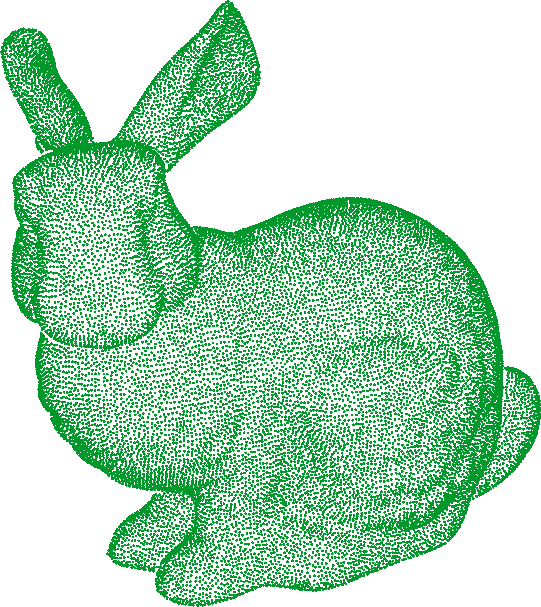
\includegraphics[height=6cm]{bunny-after-hpr}
        \caption{After the HPR.}
        \label{fig:after-hpr}
    \end{subfigure}

    \caption{Result of the HPR operator in the Bunny point cloud.}
    \label{fig:hpr-operator-bunny}

\end{figure}

\subsection{Color Attribution}

\newcommand\ceil[1]{\lceil #1 \rceil}
\newcommand\floor[1]{\lfloor #1 \rfloor}

Finally, the color is selected from the image at the pixel coordinates $(u, v)$ and saved for the correspondent pixel. Because images are discrete, the color is interpolated using a bilinear interpolation, which uses the neighbor pixels to interpolate the color $C$ at $(u, v)$ in an image $I$ according to \cref{eqn:bilinear-interpolation} (the ceil and floor operators are, respectively, $\ceil{\cdot}$ and $\floor{\cdot}$). The interpolation can be visualized in \cref{fig:bilinear-interpolation}.

\begin{equation}
    \label{eqn:bilinear-interpolation}
    \begin{aligned}
        C(u, v) = \ & (u - \ceil{u}) \ (v - \ceil{v}) \ I_{\floor{u}, \floor{v}} \\
                + \ &  (u - \ceil{u}) \ (v - \floor{v}) \ I_{\floor{u}, \ceil{v}} \\
                + \ &  (u - \floor{u}) \ (v - \ceil{v}) \ I_{\ceil{u}, \floor{v}} \\
                + \ &  (u - \floor{u}) \ (v - \floor{v}) \ I_{\ceil{u}, \ceil{v}} \\
    \end{aligned}
\end{equation}

\begin{figure}[h]
    \centering
    \begin{tikzpicture}
        \draw[-latex] (-1, -1) -- (4, -1) node[below] {$u$};
        \draw[-latex] (-1, -1) -- (-1, 4) node[left] {$v$};

        \coordinate (c00) at (0,0);
        \coordinate (c10) at (3,0);
        \coordinate (c01) at (0,3);
        \coordinate (c11) at (3,3);
        \coordinate (c) at (1.7, 1.7);

        \draw[fill] (c00) circle (0.04) node[above right, scale=0.7] {$(\floor{u}, \floor{v})$};
        \draw[fill] (c10) circle (0.04) node[above right, scale=0.7] {$(\ceil{u}, \floor{v})$};
        \draw[fill] (c01) circle (0.04) node[above right, scale=0.7] {$(\floor{u}, \ceil{v})$};
        \draw[fill] (c11) circle (0.04) node[above right, scale=0.7] {$(\ceil{u}, \ceil{v})$};

        \draw[fill] (c) circle (0.04) node[above right, scale=0.7] {$(u, v)$};

        \draw[dotted] (c00) -- (c10) -- (c11) -- (c01) -- cycle;

        \draw[dotted] (c00) -| (c) -| cycle;

    \end{tikzpicture}

    \caption{Bilinear interpolation in an image.}
    \label{fig:bilinear-interpolation}

\end{figure}


\section{Color Fusion}
\label{section:color-fusion}

In a capture with $N_a$ acquisitions, each one with $N_i$ images, the total number of images account to $N_a \times N_i$. Each one of this images will yield a partial colorized point cloud, according to \cref{section:color-registration}, and the point clouds need to be merged into a final point cloud. More specifically, each point $p_i$ has multiple correspondent colors, one for each registered image. The method here described determines the final color in a point-wise fashion and does not account for the neighbor points.

Let us admit that the point $p$ has a set $C = \{c_i|i=1\dots k\}$ of $k$ registered colors. The final color of this point $c$ should be a combination of the colors in $C$. 

The first approach is to colorize the point with one image only, for example, the first or last image. This method is the easiest and the faster, but does not consider the other images for the colorization. 

The second approach is to average the colors to obtain the color $c$, as seen in \cref{eqn:color-mean}. However, this is a poor heuristic as it considers that all colors have the same error, which is not true. For example, an image taken closer to an object is more precise than one taken away from it. 

\begin{equation}
    \label{eqn:color-mean}
    c = \frac{1}{k} \sum_{i}^{k}{c_i}
\end{equation}

A common solution for the mean limitation is to use an weighted mean, shown in \cref{eqn:weighted-mean}. The $w_i$ are the weights for each color and should reflect the quality of each color, because colors with larger weight have a larger influence in the final color.

\begin{equation}
    \label{eqn:weighted-mean}
    c = \frac{\sum_{i}^{k}{w_i c_i}}{\sum_{i}^{k}{w_i}}
\end{equation}

In this work, the quality measurement was determined based on an heuristic that depends on two factors, that are obtained in the color registration phase (\cref{section:color-registration}).

The first factor $f_1$ depends on the distance $d$ from the camera to the point and on the optimal focus point $d_f$. $f_1$ is smaller the bigger the distance between $d$ and $d_f$. The function used was the gaussian centered on $d_f$. The second factor $f_2$ depends on the distance from the pixel coordinates $(u,v)$ to the center of the optical center $(c_x, c_y)$. Again, a gaussian distribution was used to calculate $f_2$, and a bigger distance also yields a smaller $f_2$. In brief, both factors $f_1$ and $f_2$ are calculated according to \cref{eqn:heuristic-f1,eqn:heuristic-f2}. The parameters $\alpha$ and $\beta$ determine how wide the gaussian function is, so points farther from the peak point influence more or less. 

\begin{align}
    \label{eqn:heuristic-f1}
    f_1 & = \mathrm{exp}\left(-\frac{(d-d_f)^2}{2\alpha^2}\right) \\
    \label{eqn:heuristic-f2}
    f_2 & = \mathrm{exp}\left(-\frac{(u-c_x)^2 + (v-c_y)^2}{2\beta^2}\right) \\
\end{align}

The two factors are then combined into the weight $w$ factor of the color, based on a linear combination, dependent on a parameter $s$, which determines the influence of each factor, as seen on \cref{eqn:heuristic-w}. 

\begin{equation}
    \label{eqn:heuristic-w}
    w = s f_1 + (1-s) f_2
\end{equation}

In conclusion, for each point $p_i$ the color $c_i$ is attributed, based on the registered colors of each image. The fusion of all this colors is based on a weighted mean, where the weight of each color is determined by an heuristic that considers the location of the color in pixel coordinates and the distance of the point to the camera, in order to benefit points that have a better quality in the measurement, for example, points that are in focus or points that are closer to the camera center. This process is repeated for all the points of the point cloud until every point has a color (however, some points have no color registered, because no color was registered before).
